\documentclass[letterpaper,11pt,oneside,reqno]{article}

%%%%%%%%%%%%%%%%%%%%%%%%%%%%%%%%%%%%%%%%%%%%%%%%%%%%%%%%%%%%

\usepackage[pdftex,backref=page,colorlinks=true,linkcolor=blue,citecolor=red]{hyperref}
\usepackage[alphabetic,nobysame]{amsrefs}

%%%%%%%%%%%%%%%%%%%%%%%%%%%%%%%%%%%%%%%%%%%%%%%%%%%%%%%%%%%%
%main packages
\usepackage{amsmath,amssymb,amsthm,amsfonts,mathtools}
\usepackage{graphicx,color}
\usepackage{upgreek}
\usepackage[mathscr]{euscript}

%equations
\allowdisplaybreaks
\numberwithin{equation}{section}

%tikz
\usepackage{tikz}
\usetikzlibrary{shapes,arrows,positioning,decorations.markings}

%conveniences
\usepackage{array}
\usepackage{adjustbox}
\usepackage{cleveref}
\usepackage{enumerate}
\usepackage{datetime}
\usepackage{comment}

%paper geometry
\usepackage[DIV=12]{typearea}

%%%%%%%%%%%%%%%%%%%%%%%%%%%%%%%%%%%%%%%%%%%%%%%%%%%%%%%%%%%%
%draft-specific
\synctex=1
% \usepackage{refcheck,comment}

%%%%%%%%%%%%%%%%%%%%%%%%%%%%%%%%%%%%%%%%%%%%%%%%%%%%%%%%%%%%
%this paper specific
\newcommand{\ssp}{\hspace{1pt}}

%%%%%%%%%%%%%%%%%%%%%%%%%%%%%%%%%%%%%%%%%%%%%%%%%%%%%%%%%%%%
\newtheorem{proposition}{Proposition}[section]
\newtheorem{lemma}[proposition]{Lemma}
\newtheorem{corollary}[proposition]{Corollary}
\newtheorem{theorem}[proposition]{Theorem}
%%%%%%%%%%%%%%%%%%%%%%%%%%%%%%%%%%%%%%%%%%%%%%%%%%%%%%%%%%%%
\theoremstyle{definition}
\newtheorem{definition}[proposition]{Definition}
\newtheorem{remark}[proposition]{Remark}
\newtheorem{example}[proposition]{Example}
%%%%%%%%%%%%%%%%%%%%%%%%%%%%%%%%%%%%%%%%%%%%%%%%%%%%%%%%%%%%


\newenvironment{lnotes}{\section*{Notes for the lecturer}}{}
% \excludecomment{lnotes}


\begin{document}
\title{Lectures on Random Matrices
(Spring 2025)
\\Lecture 4: Semicircle law via tridiagonalization. \\Orthogonal polynomial ensembles}


\date{Wednesday, January 29, 2025\footnote{\href{https://lpetrov.cc/rmt25/}{\texttt{Course webpage}}
$\bullet$ \href{https://lpetrov.cc/rmt25/rmt25-notes/rmt2025-l04.tex}{\texttt{TeX Source}}
$\bullet$
Updated at \currenttime, \today}}



\author{Leonid Petrov}


\maketitle
\tableofcontents

\section{Recap}

Note: I did some live random matrix simulations
\href{https://lpetrov.cc/simulations/2025-01-28-goe/}{here}
and
\href{https://lpetrov.cc/simulations/2025-01-28-bbp-transition/}{here}
--- check them out. More simulations to come.

\subsection{Gaussian ensembles}

We introduced Gaussian ensembles,
and for GOE ($\beta=1$) we computed the joint eigenvalue density.
The normalization is so that the off-diagonal elements have variance $\frac{1}{2}$
and the diagonal elements have variance $1$.
Then the joint eigenvalue density is
\begin{equation*}
	p(\lambda_1,\ldots,\lambda_n)
	=
	\frac{1}{Z_n}\,
	\prod_{i=1}^n e^{-\frac{1}{2}\lambda_i^2}
	\prod_{1\le i<j\le n}(\lambda_i - \lambda_j),
	\qquad
	\lambda_1\ge \lambda_2\ge \ldots \ge \lambda_n.
\end{equation*}

\subsection{Tridiagonalization}

We showed that any real symmetric matrix \(A\) can be tridiagonalized by an orthogonal transformation \(Q\):
\[
	Q^\top\,A\,Q \;=\; T,
\]
where \(T\) is real symmetric tridiagonal, having nonzero entries only on the main diagonal and the first super-/subdiagonals:
\begin{equation*}
	T \;=\;
	\begin{pmatrix}
		 d_1 & \alpha_1 & 0 & \cdots & 0\\
		 \alpha_1 & d_2 & \alpha_2 & \cdots & 0\\
		 0 & \alpha_2 & d_3 & \ddots & \vdots\\
		 \vdots & \vdots & \ddots & \ddots & \alpha_{n-1}\\
		 0 & 0 & \cdots & \alpha_{n-1} & d_n
	\end{pmatrix}.
\end{equation*}
In the proof, each time we need to act in the orthogonal complement to the
subspace $e_1,\ldots,e_{k-1}$ (starting from $e_1$),
and apply a Householder reflection to zero out everything strictly
below the subdiagonal. (We apply the transformations like
$A\mapsto H A H^{\top}$, so that the first row transforms
in the same way as the first column of $A$).

\section{Tridiagonal random matrices}

\subsection{Distribution of the tridiagonal form of the GOE}

Applying the tridiagonalization to GOE, we obtain the following
random matrix model.

\begin{theorem}
\label{thm:DE-model}
Let \(W\) be an \(n\times n\) GOE matrix (real symmetric) with variances chosen so that each off-diagonal entry has variance \(1/2\) and each diagonal entry has variance \(1\).  Then there exists an orthogonal matrix \(Q\) such that
\[
   W \;=\; Q^\top\,T\,Q,
\]
where \(T\) is a real symmetric tridiagonal matrix
\begin{equation}
	\label{eq:tridiagonal-form}
   T \;=\; \begin{pmatrix}
         d_1 & \alpha_1 & 0 & \cdots \\
         \alpha_1 & d_2 & \alpha_2 & \ddots \\
         0 & \alpha_2 & d_3 & \ddots \\
         \vdots & \ddots & \ddots & \ddots
       \end{pmatrix},
\end{equation}
and the random variables \(\{d_i,\alpha_j\}_{1 \le i \le n,\;1\le j\le n-1}\) are mutually independent, with
\[
  d_i \,\sim\, \mathcal{N}(0,1),
  \qquad
  \alpha_j \;=\; \sqrt{\frac{\chi^2_{\,n-j}}{2}},
\]
where \(\chi^2_{\nu}\) is a chi-square distribution with \(\nu\) degrees of freedom.
\end{theorem}

\begin{remark}[Chi-square distributions]
The \emph{chi-square distribution} with \(\nu\) degrees of
freedom, denoted by \(\chi^2_{\nu}\), is a fundamental
distribution in statistics and probability theory. It arises
naturally as the distribution of the sum of the squares of
\(\nu\) independent standard normal random variables.
Formally, if \(Z_1, Z_2, \ldots, Z_{\nu}\) are independent
random variables with \(Z_i \sim \mathcal{N}(0,1)\), then
the random variable
\[
  Q = \sum_{i=1}^{\nu} Z_i^2
\]
follows a chi-square distribution with \(\nu\) degrees of
freedom, i.e., \(Q \sim \chi^2_{\nu}\). In the context of
\Cref{thm:DE-model}, the $\alpha_j$'s can be called \emph{chi random variables}.

The parameter $\nu$ does not need to be an integer, and the
chi-square distribution is well defined for any positive
real $\nu$, for example, by continuation of the density formula.
The probability density is
\begin{equation*}
	f(x) \;=\; \frac{1}{2^{\nu/2}\,\Gamma(\nu/2)}\,x^{\nu/2-1}\,e^{-x/2},
	\qquad x\ge 0.
\end{equation*}
\end{remark}

\begin{proof}[Proof of \Cref{thm:DE-model}]
	In the process of tridiagonalization,
	we apply Householder reflections.
	Note that the diagonal entries stay fixed,
	and we only change the off-diagonal entries.
	Let us consider these off-diagonal entries.

	In the first step, we apply the reflection in $\mathbb{R}^{n-1}$
	to turn the column vector $(a_{2,1},a_{3,1},\ldots,a_{n,1} )$ into
	a vector parallel to $(1,0,\ldots,0)\in \mathbb{R}^{n-1}$.
	Since the Householder reflection is orthogonal,
	it preserves lengths. So,
	\begin{equation*}
		\alpha_1=\sqrt{a_{21}^2+a_{31}^2+\cdots+a_{n1}^2},\qquad a_{i1}\sim
		\mathcal{N}(0,\dfrac{1}{2}).
	\end{equation*}
	This implies that $\alpha_1$ has the desired chi distribution.
	The distribution of the other entries is obtained similarly by the recursive
	application of the Householder reflections.

	Note that $\alpha_j$'s and $d_i$'s depend on nonintersecting
	subsets of the matrix entries, so they are independent. This completes the proof.
\end{proof}



\subsection{Dumitriu--Edelman G$\beta$E tridiagonal random matrices}

Let us define a general $\beta$ extension of the tridiagonal model for the
GOE.

\begin{definition}
	\label{def:tridiagonal-model-general-beta}
	Let $\beta>0$ be a parameter.
	The tridiagonal G$\beta$E is a random $n\times n$
	tridiagonal real symmetric
	matrix $T$ as in
	\eqref{eq:tridiagonal-form},
	where $d_i\sim \mathcal{N}(0,1)$ are independent standard Gaussians,
	and
	\begin{equation*}
		\alpha_j\sim \frac{1}{\sqrt 2}\chi_{\beta(n-j)},\qquad
		1\le j\le n-1,
	\end{equation*}
	are chi-distributed random variables.
\end{definition}

We showed that for $\beta=1$,
the G$\beta$E is the tridiagonal form of the GOE random matrix model.
The same holds for the two other classical betas:
\begin{proposition}[Without proof]
	\label{prop:tridiagonal-model-beta-classical}
	For $\beta=2$, the G$\beta$E is the tridiagonal form of the GUE random matrix model,
	which is the random complex Hermitian matrix with Gaussian entries and maximal
	independence. Similarly, for $\beta=4$,
	the G$\beta$E is the tridiagonal form of the GSE random matrix model.
\end{proposition}


Moreover, for all $\beta$, the joint eigenvalue density of G$\beta$E is
explicit:
\begin{theorem}[\cite{dumitriu2002matrix}]
	\label{thm:DE-joint-eigenvalue-density}
	Let \(T\) be a G$\beta$E matrix as in \Cref{def:tridiagonal-model-general-beta}.
	Then the joint eigenvalue density is given by
	\begin{equation*}
		p(\lambda_1,\ldots,\lambda_n)
		=
		\frac{1}{Z_{n,\beta}}\,
		e^{-\frac{1}{2}\sum_{i=1}^n \lambda_i^2}
		\prod_{1\le i<j\le n}|\lambda_i - \lambda_j|^\beta,
		\qquad
		\lambda_1\ge \lambda_2\ge \ldots \ge \lambda_n.
	\end{equation*}
\end{theorem}

This theorem is also given without proof. The proof involves
linear algebra and computation of the Jacobians of the
change of variables from the matrix entries to the
eigenvalues in the tridiagonal setting.  It can be found in
the original paper \cite{dumitriu2002matrix}.

\subsection{The case \texorpdfstring{$\beta=2$}{beta=2}}
\label{subsec:beta2-case}

For many questions involving \emph{local eigenvalue statistics},
the case \(\beta=2\) (the GUE, Gaussian Unitary Ensemble) is the most tractable.
This is because the joint density of the eigenvalues
admits a determinantal structure coming from
a \emph{square} Vandermonde factor
\(\,\prod_{i<j} (\lambda_i - \lambda_j)^2\)
and the Gaussian exponential
\(\,\exp\bigl(-\tfrac12 \sum \lambda_j^2\bigr)\).
Moreover, for \(\beta=2\), the random matrix model
and its correlation functions
can be expressed explicitly through determinants involving
\emph{orthogonal polynomials}, namely, the \emph{Hermite polynomials}.

\begin{proposition}[Joint density for GUE and orthogonal polynomials]
  \label{prop:gue-joint-density}
  Consider the GUE (Gaussian Unitary Ensemble) random matrix model, i.e.\ an
  \(n\times n\) complex Hermitian matrix whose entries
  are i.i.d.\ up to the Hermitian condition, with each
  off-diagonal entry distributed as
  \(\mathcal{N}(0,\tfrac12)+\mathrm{i}\,\mathcal{N}(0,\tfrac12)\)
  and each diagonal entry \(\mathcal{N}(0,1)\).
  The ordered eigenvalues \(\lambda_1 \ge \cdots \ge \lambda_n\)
  (or, without ordering, thought of as an unordered set)
  satisfy the joint probability density
  \begin{equation}
  	\label{eq:gue-joint-density}
    p(\lambda_1,\ldots,\lambda_n)
    \;=\;
    \frac{1}{Z_{n,2}}
    \prod_{j=1}^n e^{-\frac12 \lambda_j^2}
    \;\prod_{1\le i<j\le n} (\lambda_i - \lambda_j)^2,
  \end{equation}
  where \(Z_{n,2}\) is a normalization constant.

	Moreover, if
  \(\{\psi_k(\lambda)\}_{k=0}^\infty\)
	is the family of Hermite polynomials, orthonormal
  with respect to the measure
  \(w(\lambda)\,d\lambda = e^{-\lambda^2/2}\,d\lambda\)
  on \(\mathbb{R}\) (i.e.,
	\(\displaystyle\int_{-\infty}^{\infty} \psi_k(\lambda)\,\psi_\ell(\lambda)\,w(\lambda)\,d\lambda = \mathbf{1}_{k=\ell}\)),
  then one can also write
  \begin{equation}
  	\label{eq:gue-joint-OP}
    p(\lambda_1,\ldots,\lambda_n)
    \;=\;
		\mathrm{const}\cdot
		\det\Bigl[\psi_{j-1}(\lambda_k)e^{-\frac{\lambda_k^2}{4}}\Bigr]_{j,k=1}^n
		\;\det\Bigl[\psi_{j-1}(\lambda_k)e^{-\frac{\lambda_k^2}{4}}\Bigr]_{j,k=1}^n
  \end{equation}
	(the two determinants are identical, but let us keep this notation for future convenience).
\end{proposition}
The \emph{square determinant} structure is extremely useful.
It is
precisely the \(\beta=2\) counterpart
of the squared Vandermonde factor
\(\,\prod_{i<j}(\lambda_i-\lambda_j)^2\).


\begin{remark}[Hermite polynomials]
  There are various normalizations of Hermite polynomials.
  In random matrix theory for the Gaussian ensembles,
  we often use the \emph{probabilists' Hermite polynomials}
	(sometimes called \(\mathrm{He}_k\), but we use the notation $H_k$).
	There are various normalizations due to the factor in the exponent
	of $x^2$.

  A convenient definition for use with the weight \(e^{-x^2/2}\) is:
  \[
    H_k(x)
    \;=\;
    (-1)^k\, e^{\tfrac{x^2}{2}}
    \frac{d^k}{dx^k}
    \Bigl(e^{-\tfrac{x^2}{2}}\Bigr),
		\qquad
		k=0,1,\ldots,
  \]
  whose leading term is \(x^k\).
	Polynomials with the leading coeffient \(1\) are called \emph{monic}.
	The first few monic Hermite polynomials are
	\[
		H_0(x) = 1,\qquad
		H_1(x) = x,\qquad
		H_2(x) = x^2 - 1,\qquad
		H_3(x) = x^3 - 3x,\qquad
		H_4(x) = x^4 - 6x^2 + 3.
	\]
	The difference between $H_k$ and $\psi_k$ entering \Cref{prop:gue-joint-density}
	is in a constant normalization,
	since $H_k$ are monic but not orthonormal,
	while $\psi_k$ are orthonormal but not monic.
\end{remark}

\begin{proof}[Sketch of the determinantal representation]
  In brief, one observes that the factor
  \(\prod_{i<j}(\lambda_i - \lambda_j)\)
  is exactly the Vandermonde determinant
  \(\Delta(\lambda_1,\dots,\lambda_n)
  = \det\bigl[\lambda_k^{j-1}\bigr]_{j,k=1}^n\).
	Next, the Vandermonde determinant is also equal to
	the determinant built out of any monic family of polynomials of the corresponding
	degrees (by linear transformations), and so we get the desired
	representation.
\end{proof}

We will work with Hermite polynomials
and the determinantal structure in \Cref{prop:gue-joint-density}
in the next
\href{https://lpetrov.cc/rmt25/rmt25-notes/rmt2025-l05.pdf}{Lecture 5}).

\section{Wigner semicircle law via tridiagonalization}
\label{sec:semicircle-tridiagonal}


If $W$ is an $n\times n$ real Wigner matrix with entries of
mean zero and variance $1$ on the off-diagonal, then as
$n\to\infty$, the empirical spectral distribution (ESD) of
$W/\sqrt{n}$ converges weakly almost surely to the Wigner
semicircle distribution:
\[
  \mu_{\mathrm{sc}}(dx)
  \;=\;
  \frac{1}{2\pi}\,\sqrt{4 - x^2}\,\mathbf{1}_{|x|\le2}\,dx.
\]
We already derived this in
\href{https://lpetrov.cc/rmt25/rmt25-notes/rmt2025-l02.pdf}{Lecture 2}
by a direct combinatorial argument on the trace. Now we present another proof by using the tridiagonal form of $W$.  The argument is conceptually simpler in some steps, because the matrix is sparser (only tridiagonal).
At the same time, we will establish the Wigner
semicircle law for the general G$\beta$E case (but only Gaussian), and
thus it will apply to GUE and GSE.

%%%%%%%%%%%%%%%%%%%%%%%%%%%%%%%%%%%%%%%%%%%%%%%%%%%%%%%%%%%%
\subsection{Moments for tridiagonal matrices}
\label{sub:tridiag-moments}
%%%%%%%%%%%%%%%%%%%%%%%%%%%%%%%%%%%%%%%%%%%%%%%%%%%%%%%%%%%%

Consider
the rescaled
G$\beta$E
matrix $T/\sqrt{n}$:
\[
  \frac{T}{\sqrt{n}}
  \;=\;
  \begin{pmatrix}
    d_1/\sqrt{n} & \alpha_1/\sqrt{n} & 0 & \cdots \\
    \alpha_1/\sqrt{n} & d_2/\sqrt{n} & \alpha_2/\sqrt{n} & \ddots \\
    0 & \alpha_2/\sqrt{n} & d_3/\sqrt{n} & \ddots \\
    \vdots & \ddots & \ddots & \ddots
  \end{pmatrix},
\]
where $d_i \sim \mathcal{N}(0,1)$ and $\alpha_j \sim \frac{1}{\sqrt 2}\chi_{\beta(n-j)}$.  We want to show that the ESD of $T/\sqrt{n}$ converges to the semicircle law.
We will mostly consider expected traces of powers, and leave the analytic parts of the
argument to the reader.

The $k$-th (random) moment of the ESD
$\frac{1}{n}\sum_{i=1}^n \delta_{\lambda_i/\sqrt{n}}$ is
\begin{equation}
	\label{eq:tridiagonal-moments-expansion}
  \frac{1}{n}\operatorname{Tr}\Bigl(\tfrac{T}{\sqrt{n}}\Bigr)^k
  \;=\;
  \frac{1}{n^{1 + \frac{k}{2}}}
  \sum_{i_1,\dots,i_k=1}^n
	t_{i_1,i_2}\cdots t_{i_k,i_1},
\end{equation}
where $t_{ij}$ are the non-rescaled entries of $T$.
But now $t_{ij}$ is nonzero only if $\lvert i-j\rvert \le1$,
i.e.\ the $(i,j)$ entry is on the main or first
super-/subdiagonal.
In a closed product $t_{i_1 i_2}\cdots t_{i_k i_1}$, we thus get a \emph{closed walk} in a linear graph on the vertex set $\{1,2,\dots,n\}$ with edges only between consecutive indices.

The relevant combinatorial objects encoding these walks are
lattice walks in $\mathbb{Z}^2_{\ge0}$
starting at $(0,m)$, ending at $(k,m)$, and consisting of steps
\((1,0)\), \((1,1)\), and \((1,-1)\).  The steps \((1,0)\) correspond to
picking the diagonal element; steps
\((1,1)\) correspond to picking $i_{\ell+1}=i_\ell+1$, and
steps \((1,-1)\) correspond to $i_{\ell+1}=i_\ell-1$.
See \Cref{fig:motzkin} for an illustration of a path.
\begin{figure}[htb]
	\begin{center}
		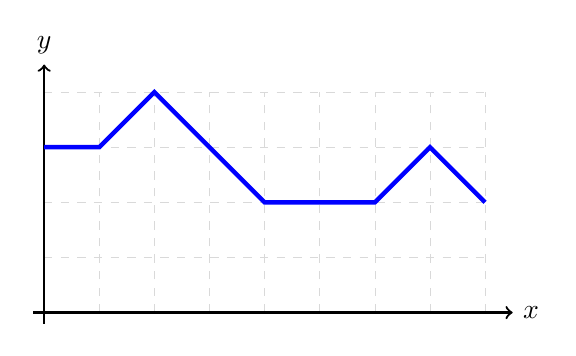
\begin{tikzpicture}[scale=0.7]
			\draw[help lines, color=gray!30, dashed] (0,0) grid (8,4);
			\draw[->,thick] (-0.2,0) -- (8.5,0) node[right] {$x$};
			\draw[->,thick] (0,-0.2) -- (0,4.5) node[above] {$y$};
			\draw[ultra thick,blue] (0,3)--++(1,0)--++(1,1)--++(2,-2)--++(2,0)--++(1,1)--++(1,-1);
		\end{tikzpicture}
	\caption{Example of a lattice path starting at height 3.}
		\label{fig:motzkin}
	\end{center}
\end{figure}

Now, each term in the sum in \eqref{eq:tridiagonal-moments-expansion}
corresponds to a path. Moreover, for each path shape,
there are $O(n)$ summands corresponding to it. The number of
paths of length $k$ starting from a fixed $m$ 
is finite (independent of $n$ for $m\gg 1$),
so we need to look more closely at the asymptotics of the product
in \eqref{eq:tridiagonal-moments-expansion}. This product
involves chi random variables which depend on $n$, too.

%%%%%%%%%%%%%%%%%%%%%%%%%%%%%%%%%%%%%%%%%%%%%%%%%%%%%%%%%%%%
\subsection{Asymptotics of chi random variables}
\label{sub:chi-asymptotics}
%%%%%%%%%%%%%%%%%%%%%%%%%%%%%%%%%%%%%%%%%%%%%%%%%%%%%%%%%%%%

One additional technical point in analyzing $T/\sqrt{n}$ is to note that $\alpha_j$
is roughly $\sqrt{\beta(n-j)/2}$ for large $n$.
Indeed, we have
\begin{equation*}
	\chi^2_\nu=\sum_{i=1}^\nu Z_i^2,\qquad
	\operatorname{\mathbb{E}}[\chi^2_\nu]=\nu,\qquad
	\operatorname{Var}[\chi^2_\nu]=2\nu.
\end{equation*}
Now, since we are dividing by $\sqrt n$, we have
\begin{equation*}
	\frac{\alpha_j}{\sqrt n}\sim \sqrt{\frac{\beta}{2}}\sqrt{1-\theta},\qquad
	\theta=\frac{j}{n}\in [0,1].
\end{equation*}
This estimate is valid in the ``bulk'' region, that is, when $\theta$ is strictly between $0$ and $1$.

Let us make these estimates more precise.  We have:
\begin{proposition}[Pointwise asymptotics in the bulk]
\label{prop:alpha-bulk}
Fix any $\delta \in (0,1)$ and let $j$ range so that $\theta_j := j/n \in [\delta,\, 1-\delta]$.
Then for each such $j$, we have\footnote{Here and below, $O_p(\cdot)$ denotes a term that is stochastically bounded at the indicated order as $n\to\infty$. That is, $X_n = O_p(a_n)$ means that for any $\epsilon>0$, there exists $M>0$ such that $\Pr(|X_n/a_n| > M) < \epsilon$ for all sufficiently large $n$.}
\[
  \frac{\alpha_j}{\sqrt{n}}
  \;=\; \sqrt{\beta\Bigl(1 - \frac{j}{n}\Bigr)}
  \;+\; O_p\Bigl(\frac{1}{\sqrt{n}}\Bigr),
\]
In particular,
\[
  \lim_{n\to\infty} \frac{\alpha_j}{\sqrt{n}}
  \;=\; \sqrt{\beta\Bigl(1-\theta_j\Bigr)}
  \quad\text{in probability.}
\]
\end{proposition}


\begin{remark}
Outside the bulk region (i.e.\ very close to $j=0$ or $j=n$), one would need a different statement to handle the case $\beta(n-j)$ is not large.
In our application, we only need the bulk behavior.
\end{remark}

Meanwhile, on the diagonal, $d_i/\sqrt{n}$
almost surely vanishes in the limit as $n\to\infty$,
because $d_i$ is standard Gaussian and does not depend on $n$.



%%%%%%%%%%%%%%%%%%%%%%%%%%%%%%%%%%%%%%%%%%%%%%%%%%%%%%%%%%%%
\subsection{Completing the proof: global semicircle behavior}
%%%%%%%%%%%%%%%%%%%%%%%%%%%%%%%%%%%%%%%%%%%%%%%%%%%%%%%%%%%%

Putting the above pieces together, we see that
\begin{equation}
	\label{eq:tridiagonal-moments-discussion}
	\frac{T}{\sqrt n}=
	\frac{1}{n}
	\sum_{i_1,\dots,i_k=1}^n
	\prod_{\ell=1}^k
	\frac{t_{i_\ell i_{\ell+1}}}{\sqrt n},\quad
	i_{k+1}=i_1 \textnormal{ by agreement}.
\end{equation}
The terms in the sum have all $i_{\ell}$'s close together
(there are $k$ indices, and they differ by $\pm1$ from each other).
We
may think that they are close to some $\theta n$, where $\theta\in [0,1]$.
We can consider only the case when $\delta<\theta<1-\delta$ for some fixed small $\delta>0$;
the case of edges does not contribute (see Problem~\ref{prob:edges-in-tridiagonal}).

If at least one of the $t_{ij}$'s in \eqref{eq:tridiagonal-moments-discussion} is
on the diagonal, the term vanishes in the limit. Therefore,
it suffices to consider only the off-diagonal $\alpha_j$'s. The
number of length $k$ walks starting from $m=\theta n$ for $\theta>\delta$ is 
just the number of lattice walks with steps $(1,\pm 1)$. This number is $\binom{k}{k/2}$.\footnote{Not Catalan yet!}
(From now on till the end of the section, we assume that
$k$ is even --- the moments become zero for odd $k$).

Fixing the starting location $\theta=\frac{i_\ell}{n}\in(\delta,1-\delta)$, we have
\begin{equation*}
	\prod_{\ell=1}^k
	\frac{t_{i_\ell i_{\ell+1}}}{\sqrt n}\to \beta^{k/2}(1-\theta)^{k/2}.
\end{equation*}

There is an extra factor $1/n$ in front in \eqref{eq:tridiagonal-moments-discussion},
which is interpreted as transforming the sum over $i_1,\ldots,i_k $
into an integral in $\theta$. We thus see that the moments converge to
\begin{equation*}
	\beta^{k/2}\binom{k}{k/2}\int_0^1 (1-\theta)^{k/2} \, d\theta=
	\beta^{k/2}\binom{k}{k/2}\cdot \frac{1}{1+k/2}, 
\end{equation*}
and we recover our favorite
Catalan moments of the semicircle distribution.

This completes the proof.

\begin{remark}[The factor $\beta^{k/2}$]
	Note that the factor $\beta^{k/2}$ refers just to the scaling of the Wigner
	semicircle law, and does not affect the semicircle shape. More precisely, 
	the limiting semicircle distribution lies from $[-2\sqrt{\beta},2\sqrt{\beta}]$.
\end{remark}

\section{Wigner semicircle law via Stieltjes transform}

Let us stay 




%!!!!!!!!!!!!!!!!!!!!!!!!!!!!!!!!!!!!!!!!!!!!!!!!!!!!!!!!!!!!!!!!!!!!!!!!!!!!!!!!!

%!!!!!!!!!!!!!!!!!!!!!!!!!!!!!!!!!!!!!!!!!!!!!!!!!!!!!!!!!!!!!!!!!!!!!!!!!!!!!!!!!
%!!!!!!!!!!!!!!!!!!!!!!!!!!!!!!!!!!!!!!!!!!!!!!!!!!!!!!!!!!!!!!!!!!!!!!!!!!!!!!!!!
%!!!!!!!!!!!!!!!!!!!!!!!!!!!!!!!!!!!!!!!!!!!!!!!!!!!!!!!!!!!!!!!!!!!!!!!!!!!!!!!!!
%!!!!!!!!!!!!!!!!!!!!!!!!!!!!!!!!!!!!!!!!!!!!!!!!!!!!!!!!!!!!!!!!!!!!!!!!!!!!!!!!!
%!!!!!!!!!!!!!!!!!!!!!!!!!!!!!!!!!!!!!!!!!!!!!!!!!!!!!!!!!!!!!!!!!!!!!!!!!!!!!!!!!
BEGIN DRAFT

%!!!!!!!!!!!!!!!!!!!!!!!!!!!!!!!!!!!!!!!!!!!!!!!!!!!!!!!!!!!!!!!!!!!!!!!!!!!!!!!!!
%!!!!!!!!!!!!!!!!!!!!!!!!!!!!!!!!!!!!!!!!!!!!!!!!!!!!!!!!!!!!!!!!!!!!!!!!!!!!!!!!!
%!!!!!!!!!!!!!!!!!!!!!!!!!!!!!!!!!!!!!!!!!!!!!!!!!!!!!!!!!!!!!!!!!!!!!!!!!!!!!!!!!
%!!!!!!!!!!!!!!!!!!!!!!!!!!!!!!!!!!!!!!!!!!!!!!!!!!!!!!!!!!!!!!!!!!!!!!!!!!!!!!!!!
%!!!!!!!!!!!!!!!!!!!!!!!!!!!!!!!!!!!!!!!!!!!!!!!!!!!!!!!!!!!!!!!!!!!!!!!!!!!!!!!!!
%%%%%%%%%%%%%%%%%%%%%%%%%%%%%%%%%%%%%%%%%%%%%%%%%%%%%%%%%%%%%%%%%%%%%%
\section{Characteristic Polynomial and Three-Term Recurrence}
\label{sec:3term}
%%%%%%%%%%%%%%%%%%%%%%%%%%%%%%%%%%%%%%%%%%%%%%%%%%%%%%%%%%%%%%%%%%%%%%

Once we have $T = (t_{ij})$ tridiagonal, the characteristic polynomial of $T$ takes a well-known form governed by a three-term recurrence. Denote
\[
  T - \lambda I \;=\;
  \begin{pmatrix}
    d_1 - \lambda & \alpha_1 & 0 & \cdots & 0 \\
    \alpha_1 & d_2 - \lambda & \alpha_2 & \cdots & 0 \\
    0        & \alpha_2 & d_3 - \lambda & \ddots & \vdots \\
    \vdots   & \vdots   & \ddots & \ddots & \alpha_{n-1} \\
    0        & 0        & \cdots & \alpha_{n-1} & d_n - \lambda
  \end{pmatrix}.
\]

\begin{definition}[Characteristic Polynomials $p_k(\lambda)$]
For $1 \le k \le n$, let $T_k$ be the top-left $k \times k$ submatrix of $T$. Define
\[
  p_k(\lambda) \;=\; \det\bigl(T_k - \lambda I_k\bigr).
\]
Moreover, set $p_0(\lambda):=1$ by convention.
\end{definition}

\begin{lemma}[Three-Term Recurrence]
\label{lem:3term-recurrence}
Let $p_k(\lambda)$ be as above, with $p_1(\lambda) = d_1 - \lambda$. Then for $k \ge 1$,
\[
  p_{k+1}(\lambda)
  \;=\;
  (d_{k+1} - \lambda)\,p_k(\lambda)
  \;-\;\alpha_k^2\,p_{k-1}(\lambda).
\]
\end{lemma}

\begin{proof}[Idea of proof]
One checks the base case $k=1,2$ directly by computing determinants of $1\times1$ and $2\times2$ blocks. For the general step, expand $\det(T_{k+1}-\lambda I_{k+1})$ by minors along the last row or column. The block structure ensures exactly the claimed recurrence.
\end{proof}

\begin{remark}
This is analogous to recurrences in orthogonal polynomials, e.g.\ the three-term recursion for polynomials orthonormal with respect to certain measures. In fact, the polynomial $p_n(\lambda)$ can be viewed as an orthogonal polynomial if $\alpha_j>0$. This interplay is vital in random matrix theory.
\end{remark}


%%%%%%%%%%%%%%%%%%%%%%%%%%%%%%%%%%%%%%%%%%%%%%%%%%%%%%%%%%%%%%%%%%%%%%
\section{Semicircle Law via the Tridiagonal Form}
\label{sec:semicircle-tridiag}
%%%%%%%%%%%%%%%%%%%%%%%%%%%%%%%%%%%%%%%%%%%%%%%%%%%%%%%%%%%%%%%%%%%%%%

We now present a fairly detailed sketch (or roadmap) for how the tridiagonal form yields the Wigner semicircle law. Recall we aim to show:

\[
  \frac{1}{n}\sum_{i=1}^n \delta_{\lambda_i/\sqrt{n}}
  \;\longrightarrow\;
  \mu_{\mathrm{sc}}(dx)\;=\;\frac{1}{2\pi}\sqrt{4 - x^2}\; 1_{|x|\le2}\,
  \quad\text{almost surely}.
\]

\subsection{The Scaling and Law of Large Numbers in \(\alpha_j\)}

Write
\[
  T = \begin{pmatrix}
    d_1 & \alpha_1 & & \\
    \alpha_1 & d_2 & \alpha_2 & \\
    & \alpha_2 & d_3 & \ddots \\
    & & \ddots & \ddots
  \end{pmatrix}.
\]
In the Dumitriu--Edelman setting, $\alpha_j^2 = \frac{1}{2}\,\chi^2_{(n-j)}$, so $ E[\alpha_j^2]=(n-j)/2$ and $\alpha_j^2$ is tightly concentrated around its mean for large $n$. Precisely, for any $\varepsilon>0$,
\[
  \Pr\Bigl(\bigl|\alpha_j^2 - \tfrac{n-j}{2}\bigr| > \varepsilon (n-j)\Bigr)
  \;\le\; e^{-c(n-j)}
\]
for some $c>0$, or a similar bound from large deviation estimates. Hence, with overwhelming probability,
\[
  \alpha_j \;\approx\; \sqrt{\frac{n-j}{2}}.
\]

\subsection{Diagonal vs.\ Subdiagonal Entries}

When we examine $\frac{1}{\sqrt{n}}\,T$, the diagonal entries become $\frac{d_i}{\sqrt{n}}$. Since $d_i \sim \mathcal{N}(0,1)$ i.i.d., with probability going to 1 these entries lie within $O(n^{-1/2})$, so they vanish in the large-$n$ limit. Meanwhile,
\[
  \frac{\alpha_j}{\sqrt{n}}
  \;\approx\;
  \sqrt{\frac{n-j}{2n}}
  \;\approx\;
  \sqrt{\frac{1 - j/n}{2}}.
\]
In the bulk region (i.e.\ $j\approx \theta n$ for $\theta\in (0,1)$), we have $\alpha_j/\sqrt{n} \approx \sqrt{\frac{1-\theta}{2}}$. In short, the subdiagonal elements (scaled by $1/\sqrt{n}$) remain of order $1$, while the diagonal elements vanish.

\subsection{Characteristic Polynomial and Recurrence Analysis}

Denote
\[
  p_n(\lambda) \;=\;
  \det\Bigl(\tfrac1{\sqrt{n}}\,T - \lambda I\Bigr).
\]
Equivalently, $\lambda$ is an eigenvalue of $\frac{1}{\sqrt{n}}\,T$ if and only if $\mu = \sqrt{n}\,\lambda$ is an eigenvalue of $T$. We want to understand the distribution of the roots $\lambda_i(\frac{1}{\sqrt{n}}\,T)$ as $n\to\infty$. The three-term recurrence for $p_n(\lambda)$ can be viewed in the limit as $n\to\infty$, turning into an integral equation for the Stieltjes transform of the limiting measure.

\paragraph{Stieltjes Transform Argument (Sketch).}
Set
\[
  G_n(z)
  = \frac{1}{n}Tr\Bigl(\bigl(\tfrac{1}{\sqrt{n}}\,T - z\Bigr)^{-1}\Bigr),
\]
the Stieltjes transform. As $n$ grows, the main input is that $\alpha_j\approx \sqrt{\frac{1-j/n}{2}}$; substituting this approximate profile into the recursion for Green’s functions (a linear difference equation akin to orthogonal polynomials) yields a limiting functional equation. Solving that equation for $G(z)$ leads to
\[
  G(z) = \frac{z \pm \sqrt{z^2-4}}{2},
\]
with the appropriate branch cut. This is the well-known Stieltjes transform for the semicircle law on $[-2,2]$. (See advanced texts, e.g.\ \emph{Deift} or \emph{Tao’s} books on RMT for a full rigorous derivation.)

\paragraph{Moment Argument (Sketch).}
One can also proceed by computing or bounding the moments $ E\bigl[\frac{1}{n}Tr(\frac{1}{\sqrt{n}}\,T)^k\bigr]$ and showing that they match the semicircle moments. Indeed, as $n\to\infty$, the diagonal part becomes negligible, while the subdiagonal structure essentially forces closed loops in the sum expansions, reproducing the Catalan numbers that appear in the Wigner moment method (Lectures 1--2). The advantage of tridiagonalization is a simpler combinatorial interpretation of the entries used in each closed loop.

\subsection{Conclusion: Wigner’s Semicircle Law}

Putting these ingredients together, we conclude that with probability 1,
\[
  \frac{1}{n}\sum_{i=1}^n \delta_{\lambda_i(\frac1{\sqrt{n}}\,W)}
  \;\;\longrightarrow\;\;
  \mu_{\mathrm{sc}}(dx) \;=\; \frac{1}{2\pi}\sqrt{4-x^2}\; 1_{|x|\le2}
\]
This completes the proof by tridiagonal methods.

\begin{remark}[Universality]
The argument here specifically used the Gaussian Wigner distribution for off-diagonal entries to get an explicit $\chi^2$ structure. However, the final result (semicircle law) remains true under vastly weaker assumptions on the entries. The \emph{universality principle} states that the global spectral behavior is insensitive to fine details of the distribution (e.g.\ it depends primarily on the first two moments).
\end{remark}







%%%%%%%%%%%%%%%%%%%%%%%%%%%%%%%%%%%%%%%%%%%%%%%%%%%%%%%%%%%%%%%%%%%%%%
\section{Exercises (Due 2025-02-28)}
\label{sec:exercises}
%%%%%%%%%%%%%%%%%%%%%%%%%%%%%%%%%%%%%%%%%%%%%%%%%%%%%%%%%%%%%%%%%%%%%%

Below are problems elaborating on the main concepts. They range from verifying computations to exploring deeper aspects of tridiagonalization and simulations.

\subsection*{1. Detailed Householder Steps and Reflection Properties}

\begin{enumerate}[(a)]
\item {\bf Constructing a Reflection that Maps One Vector to Another.}
  Let $x,y\in \mathbb{R}^n$ be nonzero. Show how to pick $v$ so that $Hx=y$, where $H=I-2\frac{v\,v^\top}{\|v\|^2}$ is a Householder reflection. Why does $H$ remain orthogonal?
\item {\bf Eliminating Below-Diagonal Entries.}
  In the first step of the tridiagonalization algorithm, pick a reflection $H_1$ that modifies the subspace spanned by $a_{21},\dots,a_{n1}$. Show explicitly how $H_1$ zeroes out all these subdiagonal entries while keeping $a_{11}$ unchanged (aside from possibly a sign).
\item {\bf Symmetry and Superdiagonal.}
  Why does $H_1 (A) H_1^\top$ also have the corresponding superdiagonal entries zeroed out in row 1? (Hint: Use $A$ is symmetric: $A_{ij}=A_{ji}$.)
\end{enumerate}

\subsection*{2. Three-Term Recurrence Warmup}

\begin{enumerate}[(a)]
\item {\bf Base Cases.} Compute $p_1(\lambda)$ and $p_2(\lambda)$ for a $2\times2$ matrix
\[
  \begin{pmatrix}
    d_1-\lambda & \alpha_1 \\
    \alpha_1 & d_2-\lambda
  \end{pmatrix}.
\]
Verify that $p_2(\lambda) = (d_2-\lambda)\,p_1(\lambda) - \alpha_1^2\,p_0(\lambda)$.
\item {\bf Inductive Step.} Using determinant expansion along the $(k+1)$-st row or column, outline why $p_{k+1}(\lambda) = (d_{k+1}-\lambda)p_k(\lambda) - \alpha_k^2 p_{k-1}(\lambda)$ for $k\ge1$.
\end{enumerate}

\subsection*{3. Tridiagonal Model for GOE and GUE}

\begin{enumerate}[(a)]
\item {\bf Real Case (GOE).} Starting with a real Wigner matrix $W$ ($X_{ij}\sim \mathcal{N}(0,1)$ for $i<j$, $X_{ii}\sim \mathcal{N}(0,2)$), show that the Householder steps produce a tridiagonal $T$ whose diagonal entries are $d_i\sim \mathcal{N}(0,1)$ and subdiagonals $\alpha_j^2 = \frac12 \chi^2_{(n-j)}$.
\item {\bf Complex Case (GUE).} For a complex Hermitian $W$, the off-diagonal entries are $\mathcal{N}(0,\tfrac12)+ i\,\mathcal{N}(0,\tfrac12)$. Sketch how the same approach yields a complex Hermitian tridiagonal form with $d_i$ real normal and $\alpha_j$ drawn from appropriate $\chi$ distributions. (You do not need a fully rigorous proof; just highlight the changes in dimension counting for real vs.\ complex parts.)
\end{enumerate}

\subsection*{4. Semicircle Law via Stieltjes Transform}

\begin{enumerate}[(a)]
\item {\bf Defining the Green’s Function.} For $z\in C\setminus\mathbb{R}$, let
\[
  G_n(z) = \frac{1}{n} \,Tr\Bigl(\bigl(\tfrac1{\sqrt{n}} T - z I\bigr)^{-1}\Bigr).
\]
Argue (informally) that $G_n(z)$ converges to a limit $G(z)$ which must satisfy an algebraic equation derived from the tridiagonal structure and the typical size of $\alpha_j$.
\item {\bf Solving for $G(z)$.} Show that $G(z)$ satisfies
\[
  G(z)^2 + z\,G(z) + 1 = 0,
\]
and deduce that
\[
  G(z) = \frac{-z + \sqrt{z^2-4}}{2}.
\]
Hence identify the imaginary part of $G(z)$ on the real interval $(-2,2)$, concluding that the limiting distribution is the semicircle law.
\end{enumerate}

\subsection*{5. Simulation of Tridiagonal vs.\ Dense Wigner}

Write a small program (in Python, MATLAB, or another language):
\begin{enumerate}[(a)]
\item Generate a dense GOE matrix $W$ of size $n=1000$ and scale by $\frac{1}{\sqrt{n}}$. Compute eigenvalues and plot a histogram.
\item Generate the corresponding tridiagonal matrix $T$ from the Dumitriu--Edelman approach (diagonal $d_i\sim \mathcal{N}(0,1)$, subdiag $\alpha_j= \sqrt{\tfrac12\,\chi^2_{n-j}}$). Compute eigenvalues of $\frac{1}{\sqrt{n}}T$ and compare histograms. They should match well with the semicircle shape for sufficiently large $n$.
\item (Optional) Investigate how large $n$ must be before the histogram looks convincingly semicircular.
\end{enumerate}

\subsection*{6. Wishart and MANOVA Exercises}

\begin{enumerate}[(a)]
\item {\bf Wishart from Data Matrix.} Generate an $n\times m$ data matrix $X$ with iid $\mathcal{N}(0,1)$. Form $W=X\,X^\top$. Plot the normalized eigenvalues $\lambda_i$ vs. the Marchenko–Pastur distribution $\mu_{MP}$ (with aspect ratio $m/n$). Discuss approximate agreement for moderate $n,m$.
\item {\bf Jacobi (MANOVA).} Let $X$ be $n\times t$ and $Y$ be $k\times t$ independent $\mathcal{N}(0,1)$. Form the matrix $M=(X\,X^\top +Y\,Y^\top)^{-1} (X\,X^\top)$ and find its eigenvalues in $[0,1]$. Plot their histogram and compare with the Jacobi Beta distribution.
\end{enumerate}

%%%%%%%%%%%%%%%%%%%%%%%%%%%%%%%%%%%%%%%%%%%%%%%%%%%%%%%%%%%%%%%%%%%%%%
\section{Further Reading and Next Steps}
%%%%%%%%%%%%%%%%%%%%%%%%%%%%%%%%%%%%%%%%%%%%%%%%%%%%%%%%%%%%%%%%%%%%%%

\begin{itemize}
\item {\bf Local Laws and Universality.} After establishing the global semicircle distribution, one may delve into local spectral laws (e.g.\ the sine kernel or GOE Tracy–Widom distribution at the edge). The \emph{local semicircle law} refines the analysis of the Green’s function in small intervals.
\item {\bf Dyson Brownian Motion.} Another approach interprets the eigenvalues as particles with logarithmic repulsion and uses stochastic differential equations to show that equilibrium distributions converge to the $\beta$-ensembles.
\item {\bf Other Ensembles.} Beyond Wigner, Wishart, and Jacobi, one finds many integrable and combinatorial random matrices (e.g.\ discrete random partitions, polynomial ensembles, random tilings). Orthogonal polynomial techniques remain central in these broader contexts.
\item {\bf References.}
  - I. Dumitriu and A. Edelman, \emph{Matrix models for beta ensembles}, J. Math. Phys., 2002.
  - T. Tao, \emph{Topics in Random Matrix Theory}, 2012.
  - P. Deift, \emph{Orthogonal Polynomials and Random Matrices}, 2000.
  - M. Mehta, \emph{Random Matrices}, 3rd ed., Elsevier, 2004.
  - T. Anderson, \emph{An Introduction to Multivariate Statistical Analysis}, for Wishart and MANOVA.
\end{itemize}


\bigskip
\noindent
\textbf{End of Lecture 4.} In this expanded lecture, we detailed how any real symmetric matrix is tridiagonalized, derived the three-term recurrence for the characteristic polynomial, and showed how this structure underlies a clean proof of Wigner’s semicircle law for random Wigner matrices. We also saw how these ideas extend to Wishart and Jacobi ensembles, bridging us toward the broader \(\beta\)-ensemble world. Upcoming lectures will further explore local eigenvalue statistics, universality results, and connections with integrable probability.





\appendix
\setcounter{section}{3}

\section{Problems (due 2025-02-28)}

\subsection{Eigenvalue density of G$\beta$E}

Read and understand the main principles of the
proof of \Cref{thm:DE-joint-eigenvalue-density}
in \cite{dumitriu2002matrix}.

\subsection{Chi-square mean and variance}

Let $X$ be a random variable with $\chi^2_\nu$ distribution. Compute the mean and variance of $X$.
(If $\nu$ is an integer, you can use the fact that $\chi^2_\nu$ is a sum of $\nu$ independent squares of standard normal random variables.
How to extend this to non-integer \(\nu\)?)

\subsection{Edge contributions in the tridiagonal moment computation}
\label{prob:edges-in-tridiagonal}

Show that the cases when the $i_{\ell}$'s are close to the edge ($\theta=0$ or $1$)
in \eqref{eq:tridiagonal-moments-discussion}
do not contribute to the limit of the moments.


\begin{lnotes}

	Add / finish up the discussion about tridiagonalization. The notes for L3 are updated, but
	mention it here.

	The reflection is mapping any vector into any other vector (unit vectors);
	Also, we apply it in $(n-1)$-dimensional space in the first pass.


\colorbox{yellow}{\parbox{.7\textwidth}{maybe make a simulation for Wishart and MANOVA in L4}}


\subsection{Characteristic Polynomial and Three-Term Recurrence}

Consider \(p_n(\lambda) = \det(T - \lambda I)\).  Because \(T\) is tridiagonal, we have the classical three-term recurrence for these characteristic polynomials:
\[
  p_0(\lambda) := 1,\quad
  p_1(\lambda) := d_1 - \lambda,
\]
\[
  p_{k+1}(\lambda)
  \;=\;
  (d_{k+1} - \lambda)\,p_k(\lambda)
  \;-\;\alpha_k^2\,p_{k-1}(\lambda),
  \quad
  (k=1,\dots,n-1).
\]
The eigenvalues of \(T\) are precisely the roots of \(p_n(\lambda)\).

\subsection{Sketch of the Semicircle Limit Proof}

We want to show that the empirical distribution
\[
  L_n
  \;=\;
  \frac{1}{n}\sum_{i=1}^n \delta_{\lambda_i}
\]
(where \(\lambda_1,\dots,\lambda_n\) are the eigenvalues of \(T\)) converges weakly to the semicircle law
\[
  \mu_{\mathrm{sc}}(dx)
  \;=\;
  \frac{1}{2\pi}\sqrt{4 - x^2}\,\mathbf{1}_{|x|\le 2}\,dx
\]
as \(n\to\infty\).  A typical outline:

\begin{enumerate}[1.]
\item \textbf{Law of Large Numbers for \(\alpha_j\).}
   Since \(\alpha_j^2 = \tfrac12\,\chi^2_{\,n-j}\) has mean \(\tfrac{n-j}{2}\), it is typically of order \(n/2\).  More precisely, for large \(n\), \(\alpha_j \approx \sqrt{\tfrac{n-j}{2}}\) with high probability.

\item \textbf{Scaling by \(\sqrt{n}\).}
   One rescales \(T\) by \(\tfrac{1}{\sqrt{n}}\).  This gives subdiagonal entries
   \[
     \frac{\alpha_j}{\sqrt{n}}
     \;\approx\;
     \sqrt{\frac{n-j}{2n}}
     \;\approx\;
     \sqrt{\frac{1 - j/n}{2}},
   \]
   while the diagonal entries become \(\tfrac{d_i}{\sqrt{n}}\), which vanish in the large-\(n\) limit.  So effectively, the subdiagonal structure drives the main spectral behavior in the bulk, producing the semicircle shape in the limit.

\item \textbf{Orthogonal Polynomial / Recurrence Analysis.}
   The polynomial \(p_n(\lambda)\) satisfies a discrete three-term recurrence whose ``continuum limit'' yields a certain integral equation (specifically the Stieltjes transform for the measure) whose solution is precisely the semicircle distribution.  In more detailed treatments, one shows that the moments or the Cauchy transform of \(L_n\) converge to that of \(\mu_{\mathrm{sc}}\).  The relevant PDE or integral equation is exactly solvable, producing the semicircle.

\end{enumerate}

Hence, with probability 1, as \(n\to\infty\), the empirical spectrum of \(\tfrac{1}{\sqrt{n}}\,W\) converges to the semicircle distribution on \([-2,2]\).  This precisely recovers \emph{Wigner’s semicircle law}.

\begin{remark}[Extensions]
A very similar approach works for the Gaussian Unitary Ensemble (\(\beta=2\)), leading to a random \emph{complex Hermitian} tridiagonal matrix.  For \(\beta=4\), there is a quaternionic block-tridiagonal model.  All of these point toward the same semicircle law for the global spectral distribution.
\end{remark}


\end{lnotes}



\bibliographystyle{alpha}
\bibliography{bib}


\medskip

\textsc{L. Petrov, University of Virginia, Department of Mathematics, 141 Cabell Drive, Kerchof Hall, P.O. Box 400137, Charlottesville, VA 22904, USA}

E-mail: \texttt{lenia.petrov@gmail.com}


\end{document}
